% move all configuration stuff into one file so we can focus on the content
\documentclass[aspectratio=169,hyperref={pdfpagelabels=false,colorlinks=true,linkcolor=white,urlcolor=lightblue},xcolor={table},t]{beamer}

%%%%%%%%%%%%%%%%%%%%%%%%%%%%%%%%%%%%%%%%%%%%%%%%%%%%%%%%%%%%%%%%%%%%%%%%%%%%%%%%%%
%%%%%%%%%%%%%%%%%%%%%%%%%%%%%%%%%%%%%%%%%%%%%%%%%%%%%%%%%%%%%%%%%%%%%%%%%%%%%%%%%%
% packages
\usepackage{pict2e}
\usepackage{epic}
\usepackage{amsmath,amsfonts,amssymb}
\usepackage{units}
\usepackage{fancybox}
\usepackage[absolute,overlay]{textpos} 
%\usepackage[table]{xcolor}
\usepackage{animate}
\usepackage{gensymb}
%\usepackage{graphicx}
%\usepackage{longtable}
\usepackage{multirow}
\usepackage{silence}
\usepackage{tikz}
\usepackage[backend=bibtex,style=ieee]{biblatex}
\AtEveryCitekey{\iffootnote{\tiny}{}}
%\addbibresource{include/references}



% fontsize
\let\Tiny=\tiny

%%%%%%%%%%%%%%%%%%%%%%%%%%%%%%%%%%%%%%%%%%%%%%%%%%%%%%%%%%%%%%%%%%%%%%%%%%%%%%%%%%
%%%%%%%%%%%%%%%%%%%%%%%%%%%%%%%%%%%%%%%%%%%%%%%%%%%%%%%%%%%%%%%%%%%%%%%%%%%%%%%%%%
% warnings
\pdfsuppresswarningpagegroup=1
\WarningFilter{biblatex}{Patching footnotes failed}
\WarningFilter{latexfont}{Font shape}
\WarningFilter{latexfont}{Some font shapes}
\WarningFilter{gensymb}{Not defining}


%%%%%%%%%%%%%%%%%%%%%%%%%%%%%%%%%%%%%%%%%%%%%%%%%%%%%%%%%%%%%%%%%%%%%%%%%%%%%%%%%%
%%%%%%%%%%%%%%%%%%%%%%%%%%%%%%%%%%%%%%%%%%%%%%%%%%%%%%%%%%%%%%%%%%%%%%%%%%%%%%%%%%
% theme & layout
\usetheme{Frankfurt}
\useinnertheme{rectangles}


%%%%%%%%%%%%%%%%%%%%%%%%%%%%%%%%%%%%%%%%%%%%%%%%%%%%%%%%%%%%%%%%%%%%%%%%%%%%%%%%%%
\setbeamertemplate{frametitle}[default][colsep=-4bp,rounded=false,shadow=false]
\setbeamertemplate{frametitle}
{%
    \nointerlineskip%
    %\vskip-0.5ex
    \begin{beamercolorbox}[wd=\paperwidth,ht=3.5ex,dp=0.6ex]{frametitle}
        \hspace*{1.3ex}\insertframetitle%
        
        \hspace*{1.3ex}\small\insertframesubtitle%
    \end{beamercolorbox}%
    \begin{textblock*}{100mm}(13.75cm,1cm)
        
\includegraphics[height=.4cm,keepaspectratio]{../shared/Logo_GTCMT_white}
    \end{textblock*}
}


%%%%%%%%%%%%%%%%%%%%%%%%%%%%%%%%%%%%%%%%%%%%%%%%%%%%%%%%%%%%%%%%%%%%%%%%%%%%%%%%%%
\setbeamertemplate{title page}[default][colsep=-4bp,rounded=false,shadow=false]
\setbeamertemplate{title page}
{
    %\begin{textblock*}{100mm}(15cm,.51cm)
            %\href{https://github.com/alexanderlerch/ACA-Slides/blob/2nd_edition/\jobname.pdf}{\includegraphics[height=.5cm,keepaspectratio]{graph/Logo_github}}\hspace*{2ex}
    %\end{textblock*}
    %\begin{textblock*}{100mm}(15cm,1.3cm)
            %\href{\IEEELink}{\includegraphics[height=.5cm,keepaspectratio]{graph/icon/book}}\hspace*{2ex}
    %\end{textblock*}
    \vskip-10ex
    \begin{beamercolorbox}[wd=\paperwidth,ht=.7\paperheight,dp=0.6ex]{frametitle} %35ex
        %\begin{flushright}
            %\href{http://www.gtcmt.gatech.edu}{
\includegraphics[height=.8cm,keepaspectratio]{graph/Logo_GTCMT_black}}\hspace*{2ex}
        %\end{flushright}
        
        \hspace*{1.8ex}\LARGE\inserttitle%
        
        \vspace*{.5ex}
        
        \hspace*{1.3ex}\small\insertsubtitle%
        
        \vspace*{.5ex}
    \end{beamercolorbox}%
    \nointerlineskip%
    \begin{beamercolorbox}[wd=\paperwidth,ht=.4\paperheight,dp=0.6ex]{page number in head/foot}
        %\vspace*{-.5ex}
        \hspace*{1.7ex}\small\insertauthor%
        
        %\hspace*{1.7ex}\small }%
        
        \vspace*{12ex}
        \vfill
        \begin{flushright}
            \href{http://www.gtcmt.gatech.edu}{
\includegraphics[height=.5cm,keepaspectratio]{../shared/Logo_GTCMT_black}}\hspace*{2ex}
        \end{flushright}
    \end{beamercolorbox}%
}


%%%%%%%%%%%%%%%%%%%%%%%%%%%%%%%%%%%%%%%%%%%%%%%%%%%%%%%%%%%%%%%%%%%%%%%%%%%%%%%%%%
%\makeatother
\setbeamertemplate{footline}
{
  \leavevmode%
  \hbox{%
  \begin{beamercolorbox}[wd=.5\paperwidth,ht=2.25ex,dp=1ex,left,leftskip=1ex]{page number in head/foot}%
    \insertsubtitle
  \end{beamercolorbox}%
  \begin{beamercolorbox}[wd=.5\paperwidth,ht=2.25ex,dp=1ex,right,rightskip=1ex]{page number in head/foot}%
    \hfill
    \insertframenumber{} / \inserttotalframenumber
  \end{beamercolorbox}}%
  \vskip0pt%
}
%\makeatletter


%%%%%%%%%%%%%%%%%%%%%%%%%%%%%%%%%%%%%%%%%%%%%%%%%%%%%%%%%%%%%%%%%%%%%%%%%%%%%%%%%%
\beamertemplatenavigationsymbolsempty
\setbeamertemplate{navigation symbols}{}
\setbeamertemplate{blocks}[default]%[rounded=false,shadow=false]
\setbeamertemplate{itemize item}[square]
\setbeamertemplate{itemize subitem}[circle]
\setbeamertemplate{itemize subsubitem}[triangle]
\setbeamertemplate{enumerate item}[square]
\setbeamertemplate{enumerate subitem}[circle]
\setbeamertemplate{enumerate subsubitem}[circle]


%%%%%%%%%%%%%%%%%%%%%%%%%%%%%%%%%%%%%%%%%%%%%%%%%%%%%%%%%%%%%%%%%%%%%%%%%%%%%%%%%%
% colors
\setbeamercolor{structure}{fg=darkgray}
\setbeamercovered{transparent} %invisible
\setbeamercolor{bibliography entry author}{fg=black}
\setbeamercolor*{bibliography entry title}{fg=black}
\setbeamercolor*{bibliography entry note}{fg=black}
\setbeamercolor{frametitle}{fg=black}
\setbeamercolor{title}{fg=white}
\setbeamercolor{subtitle}{fg=white}
\setbeamercolor{frametitle}{fg=white}
\setbeamercolor{framesubtitle}{fg=white}
\setbeamercolor{mini frame}{fg=white, bg=black}
\setbeamercolor{section in head/foot}{fg=white, bg=darkgray}
\setbeamercolor{page number in head/foot}{fg=black, bg=gtgold}
\setbeamercolor{item projected}{fg=white, bg=black}

%---------------------------------------------------------------------------------

%%%%%%%%%%%%%%%%%%%%%%%%%%%%%%%%%%%%%%%%%%%%%%%%%%%%%%%%%%%%%%%%%%%%%%%%%%%%%%%%%%
%%%%%%%%%%%%%%%%%%%%%%%%%%%%%%%%%%%%%%%%%%%%%%%%%%%%%%%%%%%%%%%%%%%%%%%%%%%%%%%%%%
% title information
\title[]{MUSI6202: Digital Signal Processing for Music}   
\author[alexander lerch]{alexander lerch} 
%\institute{~}
%\date[Alexander Lerch]{}
%\titlegraphic{\vspace{-16mm}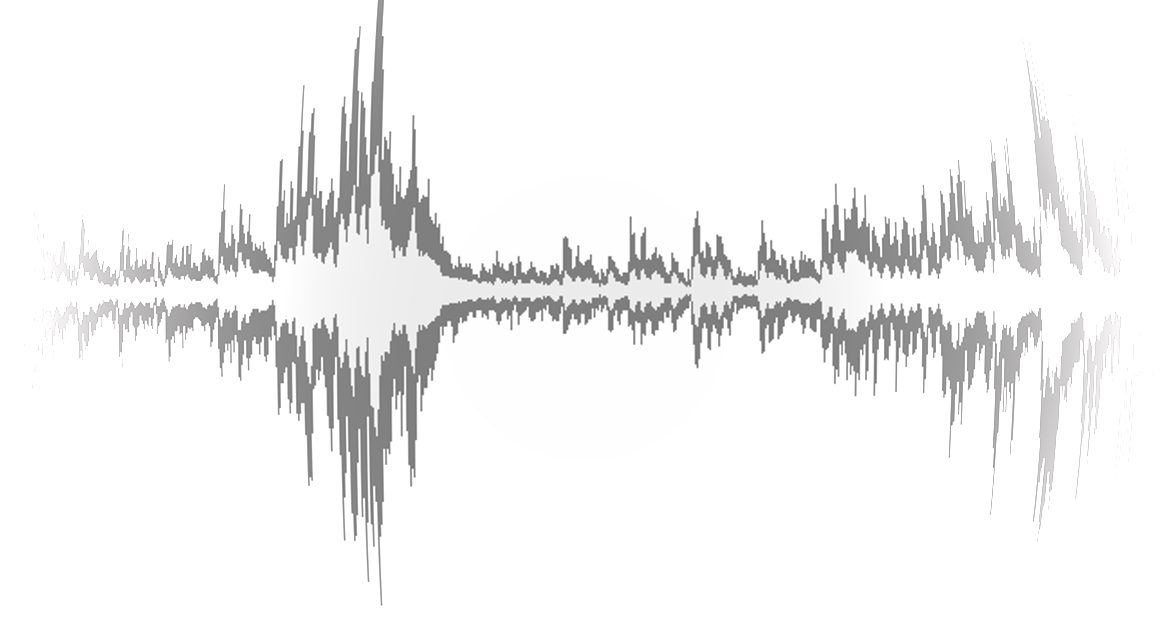
\includegraphics[width=\textwidth,height=3cm]{title}}

%%%%%%%%%%%%%%%%%%%%%%%%%%%%%%%%%%%%%%%%%%%%%%%%%%%%%%%%%%%%%%%%%%%%%%%%%%%%%%%%%%
%%%%%%%%%%%%%%%%%%%%%%%%%%%%%%%%%%%%%%%%%%%%%%%%%%%%%%%%%%%%%%%%%%%%%%%%%%%%%%%%%%
% colors
\definecolor{gtgold}{rgb}{.914, .664, 0} %0e7eed {rgb}{0.88,0.66,1,0.06} [234, 170, 0]/256 %96caff
\definecolor{darkgray}{rgb}{.15, .15, .15}
\definecolor{lightblue}{HTML}{0e7eed}
\definecolor{highlight}{rgb}{0, 0, 1} %_less!40

%%%%%%%%%%%%%%%%%%%%%%%%%%%%%%%%%%%%%%%%%%%%%%%%%%%%%%%%%%%%%%%%%%%%%%%%%%%%%%%%%%
%%%%%%%%%%%%%%%%%%%%%%%%%%%%%%%%%%%%%%%%%%%%%%%%%%%%%%%%%%%%%%%%%%%%%%%%%%%%%%%%%%
% relative paths
\graphicspath{{../graph/}}


%%%%%%%%%%%%%%%%%%%%%%%%%%%%%%%%%%%%%%%%%%%%%%%%%%%%%%%%%%%%%%%%%%%%%%%%%%%%%%%%%%
%%%%%%%%%%%%%%%%%%%%%%%%%%%%%%%%%%%%%%%%%%%%%%%%%%%%%%%%%%%%%%%%%%%%%%%%%%%%%%%%%%
% units
\setlength{\unitlength}{1mm}

%%%%%%%%%%%%%%%%%%%%%%%%%%%%%%%%%%%%%%%%%%%%%%%%%%%%%%%%%%%%%%%%%%%%%%%%%%%%%%%%%%
%%%%%%%%%%%%%%%%%%%%%%%%%%%%%%%%%%%%%%%%%%%%%%%%%%%%%%%%%%%%%%%%%%%%%%%%%%%%%%%%%%
% math
\DeclareMathOperator*{\argmax}{argmax}
\DeclareMathOperator*{\argmin}{argmin}
\DeclareMathOperator*{\atan}{atan}
\DeclareMathOperator*{\arcsinh}{arcsinh}
\DeclareMathOperator*{\sign}{sign}
\DeclareMathOperator*{\tcdf}{tcdf}
\DeclareMathOperator*{\si}{sinc}
\DeclareMathOperator*{\princarg}{princarg}
\DeclareMathOperator*{\arccosh}{arccosh}
\DeclareMathOperator*{\hwr}{HWR}
\DeclareMathOperator*{\flip}{flip}
\DeclareMathOperator*{\sinc}{sinc}
\DeclareMathOperator*{\floor}{floor}
\newcommand{\e}{{e}}
\newcommand{\jom}{\mathrm{j}\omega}
\newcommand{\jOm}{\mathrm{j}\Omega}
\newcommand   {\mat}[1]    		{\boldsymbol{\uppercase{#1}}}		%bold
\renewcommand {\vec}[1]    		{\boldsymbol{\lowercase{#1}}}		%bold

%%%%%%%%%%%%%%%%%%%%%%%%%%%%%%%%%%%%%%%%%%%%%%%%%%%%%%%%%%%%%%%%%%%%%%%%%%%%%%%%%%
%%%%%%%%%%%%%%%%%%%%%%%%%%%%%%%%%%%%%%%%%%%%%%%%%%%%%%%%%%%%%%%%%%%%%%%%%%%%%%%%%%
% media9
\newcommand{\includeaudio}[1]{
\href{run:audio/#1.mp3}{
\includegraphics[width=5mm, height=5mm]{graph/SpeakerIcon}}}

\newcommand{\includeanimation}[4]{{\begin{center}
                        \animategraphics[autoplay,loop,scale=.7]{#4}{animation/#1-}{#2}{#3}        
                        \end{center}
                        \addreference{matlab source: \href{https://github.com/alexanderlerch/ACA-Plots/blob/master/matlab/animate#1.m}{matlab/animate#1.m}}}
                        \inserticon{video}}
                        
%%%%%%%%%%%%%%%%%%%%%%%%%%%%%%%%%%%%%%%%%%%%%%%%%%%%%%%%%%%%%%%%%%%%%%%%%%%%%%%%%%
%%%%%%%%%%%%%%%%%%%%%%%%%%%%%%%%%%%%%%%%%%%%%%%%%%%%%%%%%%%%%%%%%%%%%%%%%%%%%%%%%%
% other commands
\newcommand{\question}[1]{%\vspace{-4mm}
                          \setbeamercovered{invisible}
                          \begin{columns}[T]
                            \column{.9\textwidth}
                                \textbf{#1}
                            \column{.1\textwidth}
                                \vspace{-8mm}
                                \begin{flushright}
                                     
\includegraphics[width=.9\columnwidth]{graph/question_mark}
                                \end{flushright}
                                \vspace{6mm}
                          \end{columns}\pause\vspace{-12mm}}

\newcommand{\toremember}[1]{
                        \inserticon{lightbulb}
                        }

\newcommand{\matlabexercise}[1]{%\vspace{-4mm}
                          \setbeamercovered{invisible}
                          \begin{columns}[T]
                            \column{.8\textwidth}
                                \textbf{matlab exercise}: #1
                            \column{.2\textwidth}
                                \begin{flushright}
                                     \includegraphics[scale=.5]{graph/logo_matlab}
                                \end{flushright}
                                %\vspace{6mm}
                          \end{columns}}

\newcommand{\addreference}[1]{  
                  
                    \begin{textblock*}{\baselineskip }(.98\paperwidth,.5\textheight) %(1.15\textwidth,.4\textheight)
                         \begin{minipage}[b][.5\paperheight][b]{1cm}%
                            \vfill%
                             \rotatebox{90}{\tiny {#1}}
                        \end{minipage}
                   \end{textblock*}
                    }
                    
\newcommand{\figwithmatlab}[1]{
                    \begin{figure}
                        \centering
                        \includegraphics[scale=.7]{#1}
                        %\label{fig:#1}
                    \end{figure}
                    
                    \addreference{matlab source: \href{https://github.com/alexanderlerch/MUSI-6202/blob/main/matlab/plot#1.m}{plot#1.m}}}
\newcommand{\figwithref}[2]{
                    \begin{figure}
                        \centering
                        \includegraphics[scale=.7]{#1}
                        \label{fig:#1}
                    \end{figure}
                    
                    \addreference{#2}}  
                                    
\newcommand{\inserticon}[1]{
                    \begin{textblock*}{100mm}(14.5cm,7.5cm)
                        \includegraphics[height=.8cm,keepaspectratio]{graph/#1}
                    \end{textblock*}}            

%%%%%%%%%%%%%%%%%%%%%%%%%%%%%%%%%%%%%%%%%%%%%%%%%%%%%%%%%%%%%%%%%%%%%%%%%%%%%%%%%%
%%%%%%%%%%%%%%%%%%%%%%%%%%%%%%%%%%%%%%%%%%%%%%%%%%%%%%%%%%%%%%%%%%%%%%%%%%%%%%%%%%
% counters
\newcounter{i}
\newcounter{j}
\newcounter{iXOffset}
\newcounter{iYOffset}
\newcounter{iXBlockSize}
\newcounter{iYBlockSize}
\newcounter{iYBlockSizeDiv2}
\newcounter{iXBlockSizeDiv2}
\newcounter{iDistance}

\newcommand{\IEEELink}{https://ieeexplore.ieee.org/servlet/opac?bknumber=9965970}

\addbibresource{../shared/references}



\subtitle{Part 3: Signals}

%%%%%%%%%%%%%%%%%%%%%%%%%%%%%%%%%%%%%%%%%%%%%%%%%%%%%%%%%%%%%%%%%%%%%%%%%%%%
\begin{document}
    % generate title page
	\title[]{Digital Signal Processing for Music}   
\author[alexander lerch]{alexander lerch} 
%\institute{~}
%\date[Alexander Lerch]{}
\titlegraphic{\vspace{-16mm}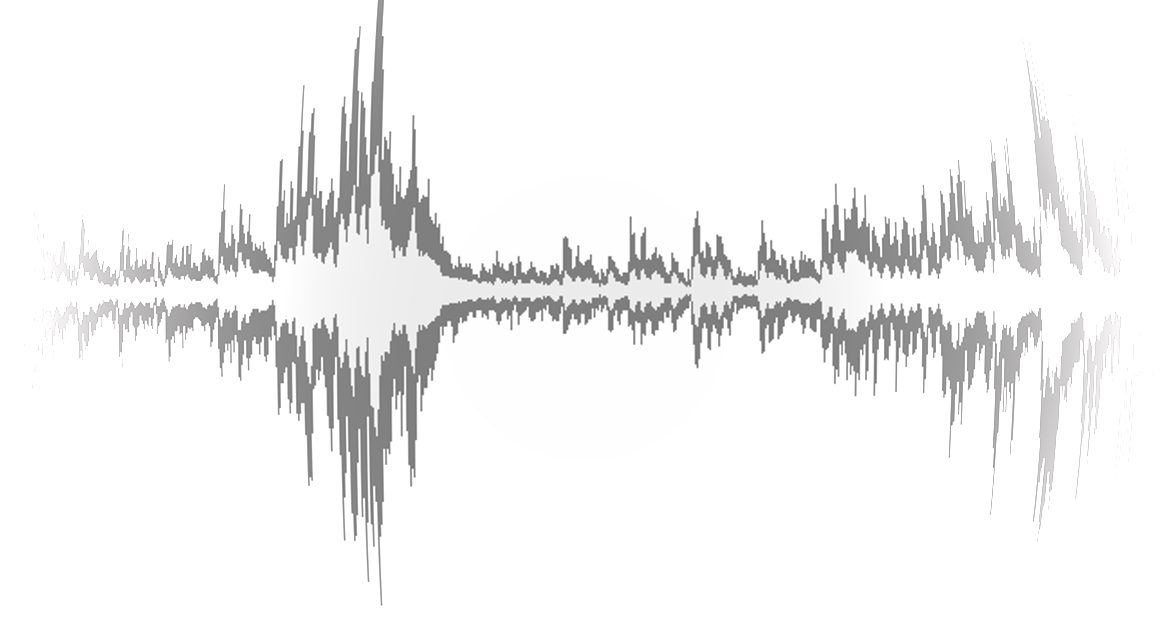
\includegraphics[width=\textwidth,height=3cm]{title}}


\begin{frame}
    \titlepage
    %\vspace{-5mm}
    \begin{flushright}
        \href{http://www.gtcmt.gatech.edu}{
\includegraphics[height=.8cm,keepaspectratio]{../shared/Logo_GTCMT_black}}
    \end{flushright}
\end{frame}


\section{introduction}
\begin{frame}{introduction}{sound}
    \begin{itemize}
        \item   sound is a vibration propagating through a medium
        \item   vibrating source excites medium and vibration is received by microphone/ear
        \item   microphone converts sound pressure (velocity) into electrical voltage
        
        \bigskip
        \item<2-> the vibration/oscillation at each of these steps is a \textbf{signal}
        \item<2-> here, we are mostly interested in the electrical signal
        
        \bigskip
        \item<3-> audio signal
            \begin{itemize}
                \item   representation of sound (speech, music, etc.)
                \item   main frequency content is below \unit[12]{kHz}
            \end{itemize}
    \end{itemize}
\end{frame}

\begin{frame}{audio signals}{categorization}
	\begin{itemize}
		\item	\textbf{deterministic signals}:\\
				\textit{predictable}: future shape of the signal can be known (example: sinusoidal)
		\pause		
		\item	\textbf{random signals}:\\
				\textit{unpredictable}: no knowledge can help to predict what is coming next (example: white noise)
	\end{itemize}
    
    \pause
    \bigskip
	
	Every ``real-world'' audio signal can be modeled as a time-varying combination of 
	\begin{itemize}
		\item	(quasi-)periodic parts
		\item	(quasi-)random parts
	\end{itemize}
\end{frame}

    \section[properties]{signal properties}
        \begin{frame}{signals}{properties of real-world signals}
            \begin{itemize}
                \item   \textbf{real-valued}:
                    \begin{itemize}
                        \item   real-world signals are usually real-valued.
                    \end{itemize}
                \item<2->   \textbf{finite}:
                    \begin{itemize}
                        \item   amplitude: $max|x(t)|<\infty$ 
                        \item<3->   energy or power:
                            \begin{eqnarray*}
                                E &=& \int\limits_{-\infty}^{\infty}{x^2(t) dt}\\
                                P &=& \lim_{T \rightarrow \infty}\frac{1}{2T}\int\limits_{-T}^{T}{x^2(t) dt}
                            \end{eqnarray*}
                    \end{itemize}
                \item<4->   \textbf{smooth}:
                    \begin{itemize}
                        \item  no ``abrupt'' changes $\rightarrow$ finite bandwidth 
                    \end{itemize}
            \end{itemize}
        \end{frame}
\section{periodic signals}
\begin{frame}{audio signals}{periodic signals 1/3}
	\vspace{-3mm}
    periodic signals most prominent examples of deterministic signals: 
    \begin{columns}
    \column{.2\linewidth}
        \begin{eqnarray}
            x(t) 	&=& x(t+T_0)\nonumber\\
            f_0 	&=& \frac{1}{T_0}\nonumber\\
            \omega_0&=& \frac{2\pi}{T_0}\nonumber
        \end{eqnarray}
	
    \column{.8\linewidth}
        \only<2>{\figwithmatlab{Sine}}
        \only<3>{\figwithmatlab{Periodic}}
    \end{columns}
\end{frame}

\begin{frame}{audio signals}{periodic signals 2/3}

    \begin{block}{reconstruction}
    	periodic signals can be reconstructed through a sum of sinusoidals at frequencies $k\cdot\omega_0$
    \end{block}
    \only<1>{\vspace{70mm}}
    \vspace{-5mm}
	\setcounter{i}{1}
	\whiledo{\value{i}<6}	
	{
		\pause
		\only<\value{beamerpauses}>
		{
        
        
            \only<2>{
            \begin{equation}\nonumber
                \hat{x}(t) = a_1\cdot sin(\omega_0 t)
            \end{equation}}
            \only<3>{
            \begin{equation}\nonumber
                \hat{x}(t) = a_1\cdot sin(\omega_0 t) + a_2\cdot sin(2\cdot\omega_0 t)+\ldots+ a_{3}\cdot sin(3\cdot\omega_0 t)
            \end{equation}}
            \only<4>{
            \begin{equation}\nonumber
                \hat{x}(t) = a_1\cdot sin(\omega_0 t) + a_2\cdot sin(2\cdot\omega_0 t)+\ldots+ a_{10}\cdot sin(10\cdot\omega_0 t)
            \end{equation}}
            \only<5>{
            \begin{equation}\nonumber
                \hat{x}(t) = a_1\cdot sin(\omega_0 t) + a_2\cdot sin(2\cdot\omega_0 t)+\ldots+ a_{25}\cdot sin(25\cdot\omega_0 t)
            \end{equation}}
            \only<6>{
            \begin{equation}\nonumber
                \hat{x}(t) = a_1\cdot sin(\omega_0 t) + a_2\cdot sin(2\cdot\omega_0 t)+\ldots+ a_{50}\cdot sin(50\cdot\omega_0 t)
            \end{equation}}
			\vspace{-10mm}
            \begin{columns}
            \column{.9\linewidth}
                \begin{figure}
                    \centering
                    \includegraphics[scale=.75]{AdditiveSynthesisSaw-\arabic{i}}
                \end{figure}
            \column{.1\linewidth}
                
                \bigskip
                \only<2>{\includeaudio{additivesynthesis_saw_1} }
                \only<3>{\includeaudio{additivesynthesis_saw_2} }
                \only<4>{\includeaudio{additivesynthesis_saw_3} }
                \only<5>{\includeaudio{additivesynthesis_saw_4} }
                \only<6>{\includeaudio{additivesynthesis_saw_5} }
            \end{columns}
            \addreference{{matlab source: \href{https://github.com/alexanderlerch/MUSI-6202/blob/master/matlab/plotAdditiveSynthesis.m}{plotAdditiveSynthesis.m}}}
		}
		\stepcounter{i} 
	}	
	\setcounter{i}{1}
	\whiledo{\value{i}<6}	
	{
		\pause
		\only<\value{beamerpauses}>
		{
        
            \only<7>{
            \begin{equation}\nonumber
                \hat{x}(t) = a_1\cdot sin(\omega_0 t)
            \end{equation}}
            \only<8>{
            \begin{equation}\nonumber
                \hat{x}(t) = a_1\cdot sin(\omega_0 t) + a_3\cdot sin(3\cdot\omega_0 t)+\ldots+ a_{5}\cdot sin(5\cdot\omega_0 t)
            \end{equation}}
            \only<9>{
            \begin{equation}\nonumber
                \hat{x}(t) = a_1\cdot sin(\omega_0 t) + a_3\cdot sin(3\cdot\omega_0 t)+\ldots+ a_{19}\cdot sin(19\cdot\omega_0 t)
            \end{equation}}
            \only<10>{
            \begin{equation}\nonumber
                \hat{x}(t) = a_1\cdot sin(\omega_0 t) + a_3\cdot sin(3\cdot\omega_0 t)+\ldots+ a_{49}\cdot sin(49\cdot\omega_0 t)
            \end{equation}}
            \only<11>{
            \begin{equation}\nonumber
                \hat{x}(t) = a_1\cdot sin(\omega_0 t) + a_3\cdot sin(3\cdot\omega_0 t)+\ldots+ a_{99}\cdot sin(99\cdot\omega_0 t)
            \end{equation}}
            \vspace{-10mm}
            \begin{columns}
            \column{.9\linewidth}
                \begin{figure}
                    \centering
                    \includegraphics[scale=.75]{AdditiveSynthesisRect-\arabic{i}}
                \end{figure}
            \column{.1\linewidth}
                
                \bigskip
                \only<7>{\includeaudio{additivesynthesis_rect_1} }
                \only<8>{\includeaudio{additivesynthesis_rect_2} }
                \only<9>{\includeaudio{additivesynthesis_rect_3} }
                \only<10>{\includeaudio{additivesynthesis_rect_4} }
                \only<11>{\includeaudio{additivesynthesis_rect_5} }
            \end{columns}
            \addreference{{matlab source: \href{https://github.com/alexanderlerch/MUSI-6202/blob/master/matlab/plotAdditiveSynthesis.m}{plotAdditiveSynthesis.m}}}
		}
		\stepcounter{i} 
	}	
\end{frame}

\begin{frame}{audio signals}{periodic signals 3/3}
    youtube --- mechanical additive synthesis:
    
    \url{http://youtu.be/8KmVDxkia_w}
    
\end{frame}


\begin{frame}{audio signals}{superposition of sinusoidals 1/2}
    \begin{itemize}
        \item   \textbf{partials}:\\ a set of frequencies comprising a (pitched) sound
        \bigskip
        \item   \textbf{overtones}:\\ as partials but without the fundamental frequency
        \bigskip
        \item   \textbf{harmonics}:\\ integer multiples of the fundamental frequency, including the fundamental frequency
    \end{itemize}
    
    %\pause
    %\bigskip
    %\toremember{all periodic signals ...}
    %\begin{itemize}
        %\item   have fundamental frequency (even if weight might be zero)
        %\item   consist  only of sinusoidals at integer multiples of fundamental frequency
    %\end{itemize}
\end{frame}

\begin{frame}{audio signals}{superposition of sinusoidals 2/2}
    \vspace{-6mm}
    \begin{footnotesize}
        \begin{eqnarray*}
            y(t) &=& \underbrace{\sin\left(2\pi (f+\frac{\Delta f}{2})t\right)}_{\sin(2\pi f)\cos\left(2\pi t\frac{\Delta f}{2}\right) + \cos(2\pi f)\sin\left(2\pi t\frac{\Delta f}{2}\right)} + \underbrace{\sin\left(2\pi (f-\frac{\Delta f}{2})t\right)}_{\sin(2\pi f)\cos\left(-2\pi t\frac{\Delta f}{2}\right) + \cos(2\pi f)\sin\left(-2\pi t\frac{\Delta f}{2}\right)}\\
          &=& 2\sin\left(2\pi f\right)\cdot \cos\left(2\pi\frac{\Delta f}{2}t\right)
        \end{eqnarray*}
    \only<1>{
        \vspace{-3mm}
        \figwithmatlab{Beating}
    }
    \only<2>{
    
    \bigskip
    \bigskip
    {\normalsize audio examples: addition of sines}
    \begin{table}
        \centering
            \begin{tabular}{l|ccccccccc}
                $500\unit{Hz}$ & $+1000$ & $+750$ & $+667$ & $+625$ & $+600$ &$+530$ &$+502$ &$+501$\\
                \includeaudio{Beating_sine}& \includeaudio{Beating_1000}& \includeaudio{Beating_750}& \includeaudio{Beating_667}& \includeaudio{Beating_625}& \includeaudio{Beating_600}& \includeaudio{Beating_530}& \includeaudio{Beating_502}& \includeaudio{Beating_501} \\
            \end{tabular}
    \end{table}
     }
    \end{footnotesize}
    \vspace{30mm}
\end{frame}

\section{random signals}	
\begin{frame}{audio signals}{random process}
	\textbf{random process}: ensemble of random series
    \begin{columns}
    \column{.6\linewidth}
    \vspace{-5mm}
    \figwithmatlab{RandomProcess}
	%\begin{figure}
		%\centering
			%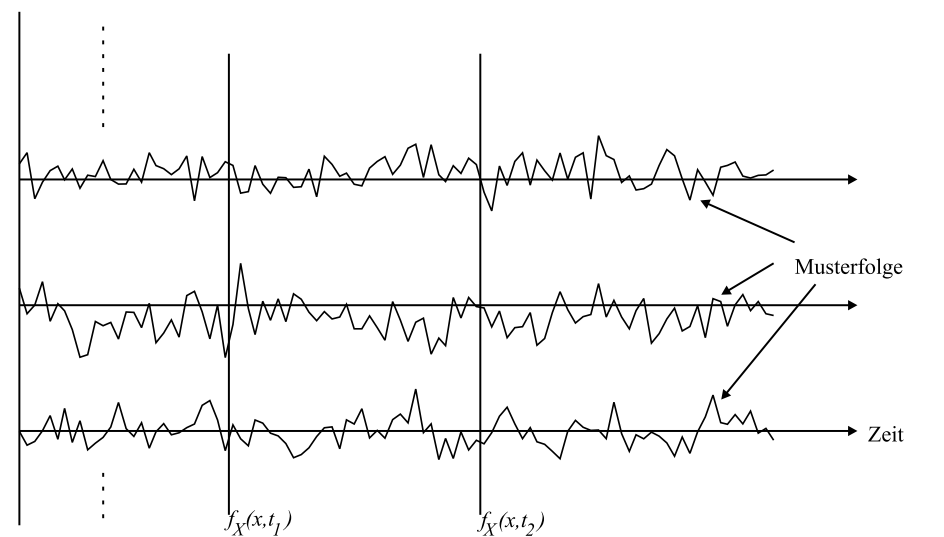
\includegraphics[scale=.25]{graph/randomprocess}
	%\end{figure}
    \column{.4\linewidth}
	special cases:
	\begin{itemize}
		\item	\textbf{stationarity}:\\ all parameters (such as the mean) are time invariant
		\bigskip
        \item	\textbf{ergodicity}:\\ process with equal time and ensemble mean (implies stationarity)
	\end{itemize}
    \end{columns}
\end{frame}

\section{prototype signals}

\begin{frame}{deterministic prototype signals}{periodic signals}
            \begin{itemize}
                \item   \textbf{sinusoidal}
                    \[x(t) = \sin(\underbrace{2\pi f}_{\omega} t {\color{gray}{+ \Phi}})\]
                \smallskip
                \item<2->   \textbf{sawtooth}
                    \begin{equation*}
                        x(t) = 2\left(\frac{t}{T_0}-\floor\left(\frac{1}{2}+\frac{t}{T_0}\right)\right)
                    \end{equation*}
                \smallskip
                \item<3->   \textbf{square wave}
                    \[x(t) = \sign\left(\sin(\omega t)\right)\]
            \end{itemize}
\end{frame}
\begin{frame}{deterministic prototype signals}{non-periodic deterministic signals}
    \begin{itemize}
        \item   \textbf{DC}
            \[ x(t) = 1\]
        \smallskip
        \item<2->   \textbf{impulse}
            \begin{equation*}
                \delta(t) = 
                    \begin{cases}
                            \infty & t = 0 \\
                            0   & t \neq 0
                    \end{cases}
            \end{equation*}
            \begin{equation*}
                \delta(t) = \int\limits_{-\infty}^{\infty}{\delta(t) dt = 1}
            \end{equation*}
        \smallskip
        \item<3->   \textbf{exponential}
            \[ x(t) = \e^{-\alpha t}\]
    \end{itemize}
\end{frame}
%\begin{frame}{non-deterministic prototype signals}{non-periodic signals}
    %\begin{itemize}
        %\item   white noise
            %\begin{itemize}
                %\item   completely random: no possibility of predicting the event
                %\item<2-> but: if noise is stationary (doesn't change over time), then signal properties are predictable
                    %\begin{itemize}
                        %\item mean \[ m = \int\limits_{\infty}^{\infty}{x(t) dt}\]
                        %\item   power
                    %\end{itemize}
            %\end{itemize}
    %\end{itemize}
%\end{frame}

\section{summary}
    \begin{frame}{audio signals}{summary}
        \begin{itemize}
            \item   two basic signal classes, \textbf{deterministic} and \textbf{random}
            \bigskip
            \item   \textit{deterministic} signals can be described by a function and are predictable
                \begin{itemize}
                    \item   special case: periodic signals --- sum of sinusoidals with freq. integer ratio
                \end{itemize}
            \bigskip
            \item   \textit{random signals} are not predictable
                \begin{itemize}
                    \item   special case: ergodic signals can be described statistically 
                \end{itemize}
        \end{itemize}
    \end{frame}
    
\end{document}

